Urban areas are highly complex environments which introduce numerous challenges
to autonomous service robots. In particular, for a safe and reliable navigation,
a robot should be able to accurately detect curbs. Curbs usually appear at the
borders between streets and sidewalks. The knowledge of curb positions and
characteristics can beneficially enhance metric maps with traversability
information relevant to navigation. For instance, depending on its physical
capabilities, a robotic platform could only drive harmlessly over curbs of a
given height when crossing a street.

Amongst the difficulties related to this task, curbs might exhibit various
curvatures and heights, and be perceived from different viewpoints. In contrast
to autonomous cars, pedestrian robots can indeed make few assumptions about
the structure of the environment. Furthermore, the sensing device noise model
should be introduced to distinguish between real curbs and measurement noise.
Ideally, the algorithm should run on-line and in real-time.

In this paper, we devise an unsupervised method to curb detection that covers
most of the aforementioned requirements. Our approach attempts to construct a
piecewise planar model of the environment and determines curbs at plane segment
boundaries. Initially, we sense the environment with a nodding laser
range-finder and project the 3D measurements into an efficient Digital Elevation
Map (DEM). Each cell of the DEM maintains an error model that is propagated
throughout the entire algorithm. Plane segments are further estimated with a
mixture of linear regression model. Here, we propose an original formulation of
the standard Expectation-Maximization (EM) algorithm for mixture models.
Specifically, in the E-step, the responsibilities are computed with a
Conditional Random Field (CRF) that introduces dependencies between the
covariates of the mixture model. A graph-based segmentation of the DEM provides
an estimate of the number of planes and initial parameters for the EM.
Sequential and fast estimations of DEM patches in the surrounding of the sensor
while the robot drives ensure on-line operation. Fig.~\ref{fig:intro} shows a
typical output of our algorithm with the curb points reprojected on the original
data.

\begin{figure}[t]
\centering
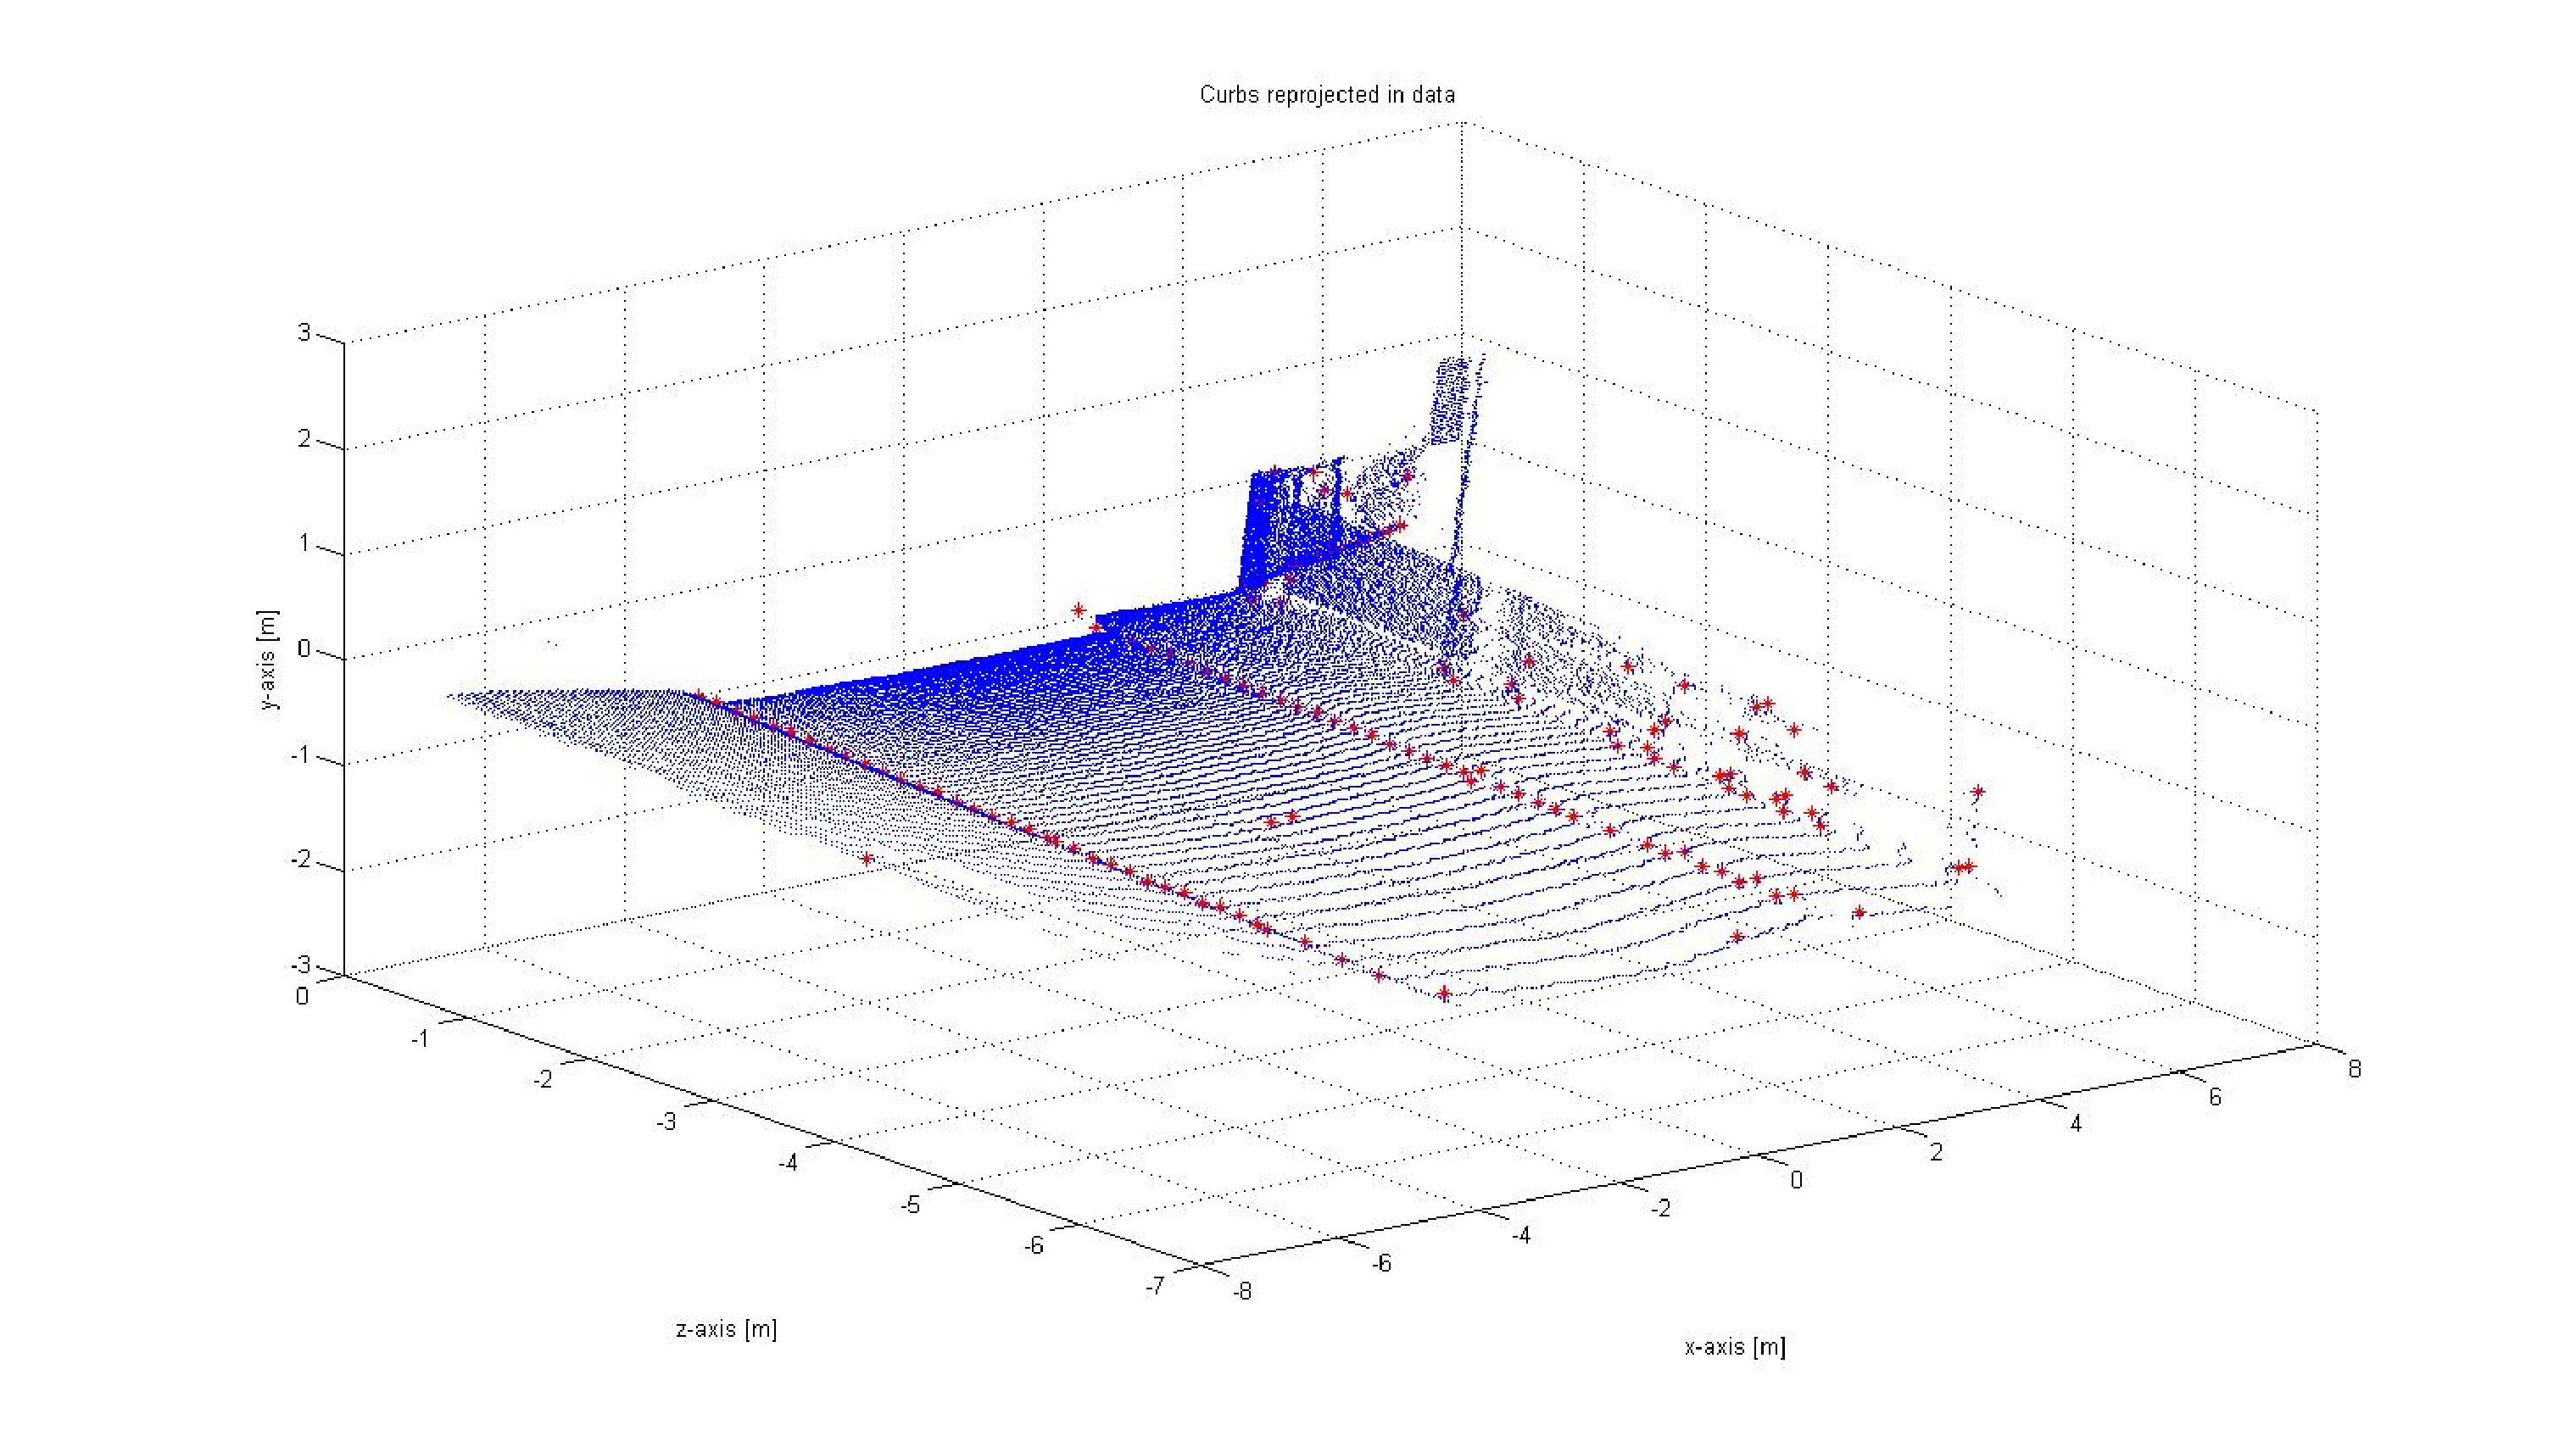
\includegraphics[width=\columnwidth]{fig/intro.eps}
\caption{Exemplary output of our curb detection algorithm. Curb points
(red stars) are reprojected into the original point cloud.}
\label{fig:intro}
\end{figure}

Clearly, the main contribution of the paper is its strict probabilistic
interpretation from the sensing process to the final plane estimation and
segmentation. Moreover, our method is view-independent and requires no
particular prior knowledge about the environment. The set of free parameters
is solely related to the sensor characteristics and involves no hand-tuning.
Finally, a direct implementation of the algorithm from the paper should be
straightforward.

The remainder of the paper is structured as follows. Section~\ref{sec:related}
summarizes the previous works related to ours. Section~\ref{sec:model}
introduces our statistical models and derives the related inference methods.
Section~\ref{sec:implementation} is concerned with implementation and
algorithmic details. Section~\ref{sec:exp} demonstrates the validity of the
method through extensive qualitative and quantitative analysis.
Section~\ref{sec:conc} outlines our conclusions and provides some insights for
future work.
